%%%%%%%%%%%%%%%%%%%MAIN_OPTIONS%%%%%%%%%%%%%%%%%%%
\documentclass[a4paper, 14pt]{article}

%% Работа с русским языком
\usepackage{cmap}					% поиск в PDF
\usepackage{hyperref}				% гиперссылки
\usepackage[warn]{mathtext} 		% русские буквы в формулах
\usepackage[T2A]{fontenc}			% кодировка
\usepackage[utf8]{inputenc}			% кодировка исходного текста
\usepackage[english,russian]{babel}	% локализация и переносы

%% Дополнительная работа с математикой
\usepackage{amsfonts,amssymb,amsthm,mathtools} % AMS
\usepackage{amsmath}
\usepackage{icomma} % "Умная" запятая: $0,2$ --- число, $0, 2$ --- перечисление

%% Номера формул
%\mathtoolsset{showonlyrefs=true} % Показывать номера только у тех формул, на которые есть \eqref{} в тексте.

%%FONTS_Packadges
\usepackage{euscript} % Шрифт Евклид
\usepackage{mathrsfs} % Красивый матшрифт

%% Свои команды
\DeclareMathOperator{\sgn}{\mathop{sgn}}

%% Перенос знаков в формулах (по Львовскому)
\newcommand*{\hm}[1]{#1\nobreak\discretionary{}
	{\hbox{$\mathsurround=0pt #1$}}{}}

%%% Работа с картинками
\usepackage{graphicx}  % Для вставки рисунков
\graphicspath{{pictures/}{images2/}}  % папки с картинками
\setlength\fboxsep{3pt} % Отступ рамки \fbox{} от рисунка
\setlength\fboxrule{1pt} % Толщина линий рамки \fbox{}
\usepackage{wrapfig} % Обтекание рисунков и таблиц текстом
\usepackage[section]{placeins}
\usepackage{subcaption}

%% Работа с таблицами
\usepackage{array,tabularx,tabulary,booktabs} % Дополнительная работа с таблицами
\usepackage{longtable}  % Длинные таблицы
\usepackage{multirow} % Слияние строк в таблице

%%Links
\hypersetup{
	colorlinks=true,
	linkcolor=black,
	filecolor=magenta,      
	urlcolor=blue,
}

%%% Программирование
\usepackage{etoolbox} % логические операторы

%%% Страница
\usepackage{extsizes} % Возможность сделать 14-й шрифт
\usepackage{geometry} % Простой способ задавать поля
\geometry{top=25mm}
\geometry{bottom=35mm}
\geometry{left=20mm}
\geometry{right=20mm}
\usepackage{indentfirst}
%
\usepackage{fancyhdr} % Колонтитулы
\pagestyle{fancy}
\renewcommand{\headrulewidth}{0mm}  % Толщина линейки, отчеркивающей верхний колонтитул
%\lfoot{Нижний левый}
%\rfoot{Нижний правый}
%\rhead{Верхний правый}
%\chead{Верхний в центре}
%\lhead{Верхний левый}
% \cfoot{Нижний в центре} % По умолчанию здесь номер страницы

\usepackage{setspace} % Интерлиньяж
%\onehalfspacing % Интерлиньяж 1.5
%\doublespacing % Интерлиньяж 2
%\singlespacing % Интерлиньяж 1

\usepackage{multicol,caption}

\newenvironment{Figure}
{\par\medskip\noindent\minipage{\linewidth}}
{\endminipage\par\medskip}

\usepackage{enumitem}
\usepackage{amssymb}
\usepackage{xcolor}
%%% Зачеркнутый текст
\usepackage[normalem]{ulem}
\usepackage{xurl}



\begin{document}

	\title{		\textbf{\textit{Победит \#398}} 
		
	Анализ микроструктур сплава WC-Co}

	\author{$ Д.Г. Каграманян^1, Д.Ю. Камалова^2, Б.Б. Страумал^3, Л.Н. Щур^4$}
	\date{\today}
	\maketitle

	\hfill
	\begin{minipage}{1\textwidth}
			\flushleft
	    $^1$исследователь,dgkagramanyan@edu.hse.ru\\
	    $^2$исследователь,dyukamalova@edu.hse.ru \\
	    $^3$соруководитель,straumal@issp.ac.ru\\
   	 	$^4$руководитель,levshchur@gmail.com\\



	\end{minipage}%

	\section{Аннотация}
	В строительстве и горнодобывающей области для инструментов и тяжелой техники зачастую используются оснатки  с твердосплавным покрытием. 
	Сплав WC-Co  - популярный твердый сплав, использующийся в задачах сверления и бурения. Хоть эта связка давно известна, еще не проводились исследования с целью определить есть ли между зависимости между физическими характеристиками сплава и ,если есть, то какие. 

	\section{Постановка задачи}
	Цель проекта - провести глубокий анализ изображения микростркутур сплава WC-Co и исследовать наличие скрытых зависимостей между характеристиками при помощи глубокого обучения. 
		
	Успешное выполнение проекта включает в себя следующие задачи
	\begin{itemize}
		\item исследование снимков микроструктур сплава;
		
		\item разработка методики для автоматической обработки изображений;
		
		\item обучение модели нейронной сети и обработка ее результатов.
	\end{itemize}
	
	\section{Планируемый результат}
		Методика обработки изоражений, исследование зависимостей характеристик сплава, публикация работы. 
	 
	 \section{Методы исследования}
	 
	 		\begin{itemize}
	 		\item анализ состава и визуальный осмотр;
	 		
	 		\item растровая обработка изображений (computer vision).
	 		
	 	\end{itemize}
	 
	 \section{Ход работ} 
		Каграманян Давид - разработчик,исследователь. Задачи
		\begin{itemize}
			\item применение и анализ популярных методов сегментации зерен сплава - \textbf{выполнено};
			
			\item разработка и анализ графовых алгоритмов для сегментации зерен и связующего вещества сплава - \textbf{выполнено};
			
			\item разработка и анализ алгоритмов для сбора геометрии сплава - \textbf{в работе}.
		\end{itemize}
	 	
	 	Камалова Даяна - исследователь. Задачи
	 	
	 	\begin{itemize}
	 		\item анализ влияния субмикронных размера зерна на механические свойства высокоэнтропийной карбидной керамики - \textbf{выполнено};
	 		
	 		\item анализ углов контакта границ зерен карбида вольфрама - \textbf{выполнено};
	 		
	 		\item изучение различных алгоритмов сегментации и подсчёта количества зёрен - \textbf{выполнено};
	 			
	 		\item анализ диаграммы состояния карбида вольфрама кобальтовой связки - \textbf{в работе}.
	 		
	 	\end{itemize}



	\section{Анализ предметной области }
	
	\subsection{Исследование исходных данных}
	Наше исследование проводится в кооперации с МИСиС (Москва) и организацией Element Six GmBH (Германия), предоставляющей нам образцы сплава. Объектом исследований в нашем 		проекте являются металлокерамические твердые сплавы Wc-Co состоящие из керамической фазы, карбида вольфрама и кобальтовой связки. В качестве входных данных мы принимали микроструктуры которые были оцифрованы в МИСиС с помощью оборудования Vega Tescan. Микроскоп с термоэмиссионным вольфрамовым катодом, позволяющий получать СЭМ-изображения и проводить анализ элементного состава в реальном времени. На каждой фотографии присутствует линейка. Ее длина для данного микроскопа 50 µм. На рисунке \ref{original} приведены примеры микроструктур, которые мы получили. Изображение слева получено на основе отраженных электронов, а справа – на поглощенных.
	
	\begin{figure}[h]
		\center{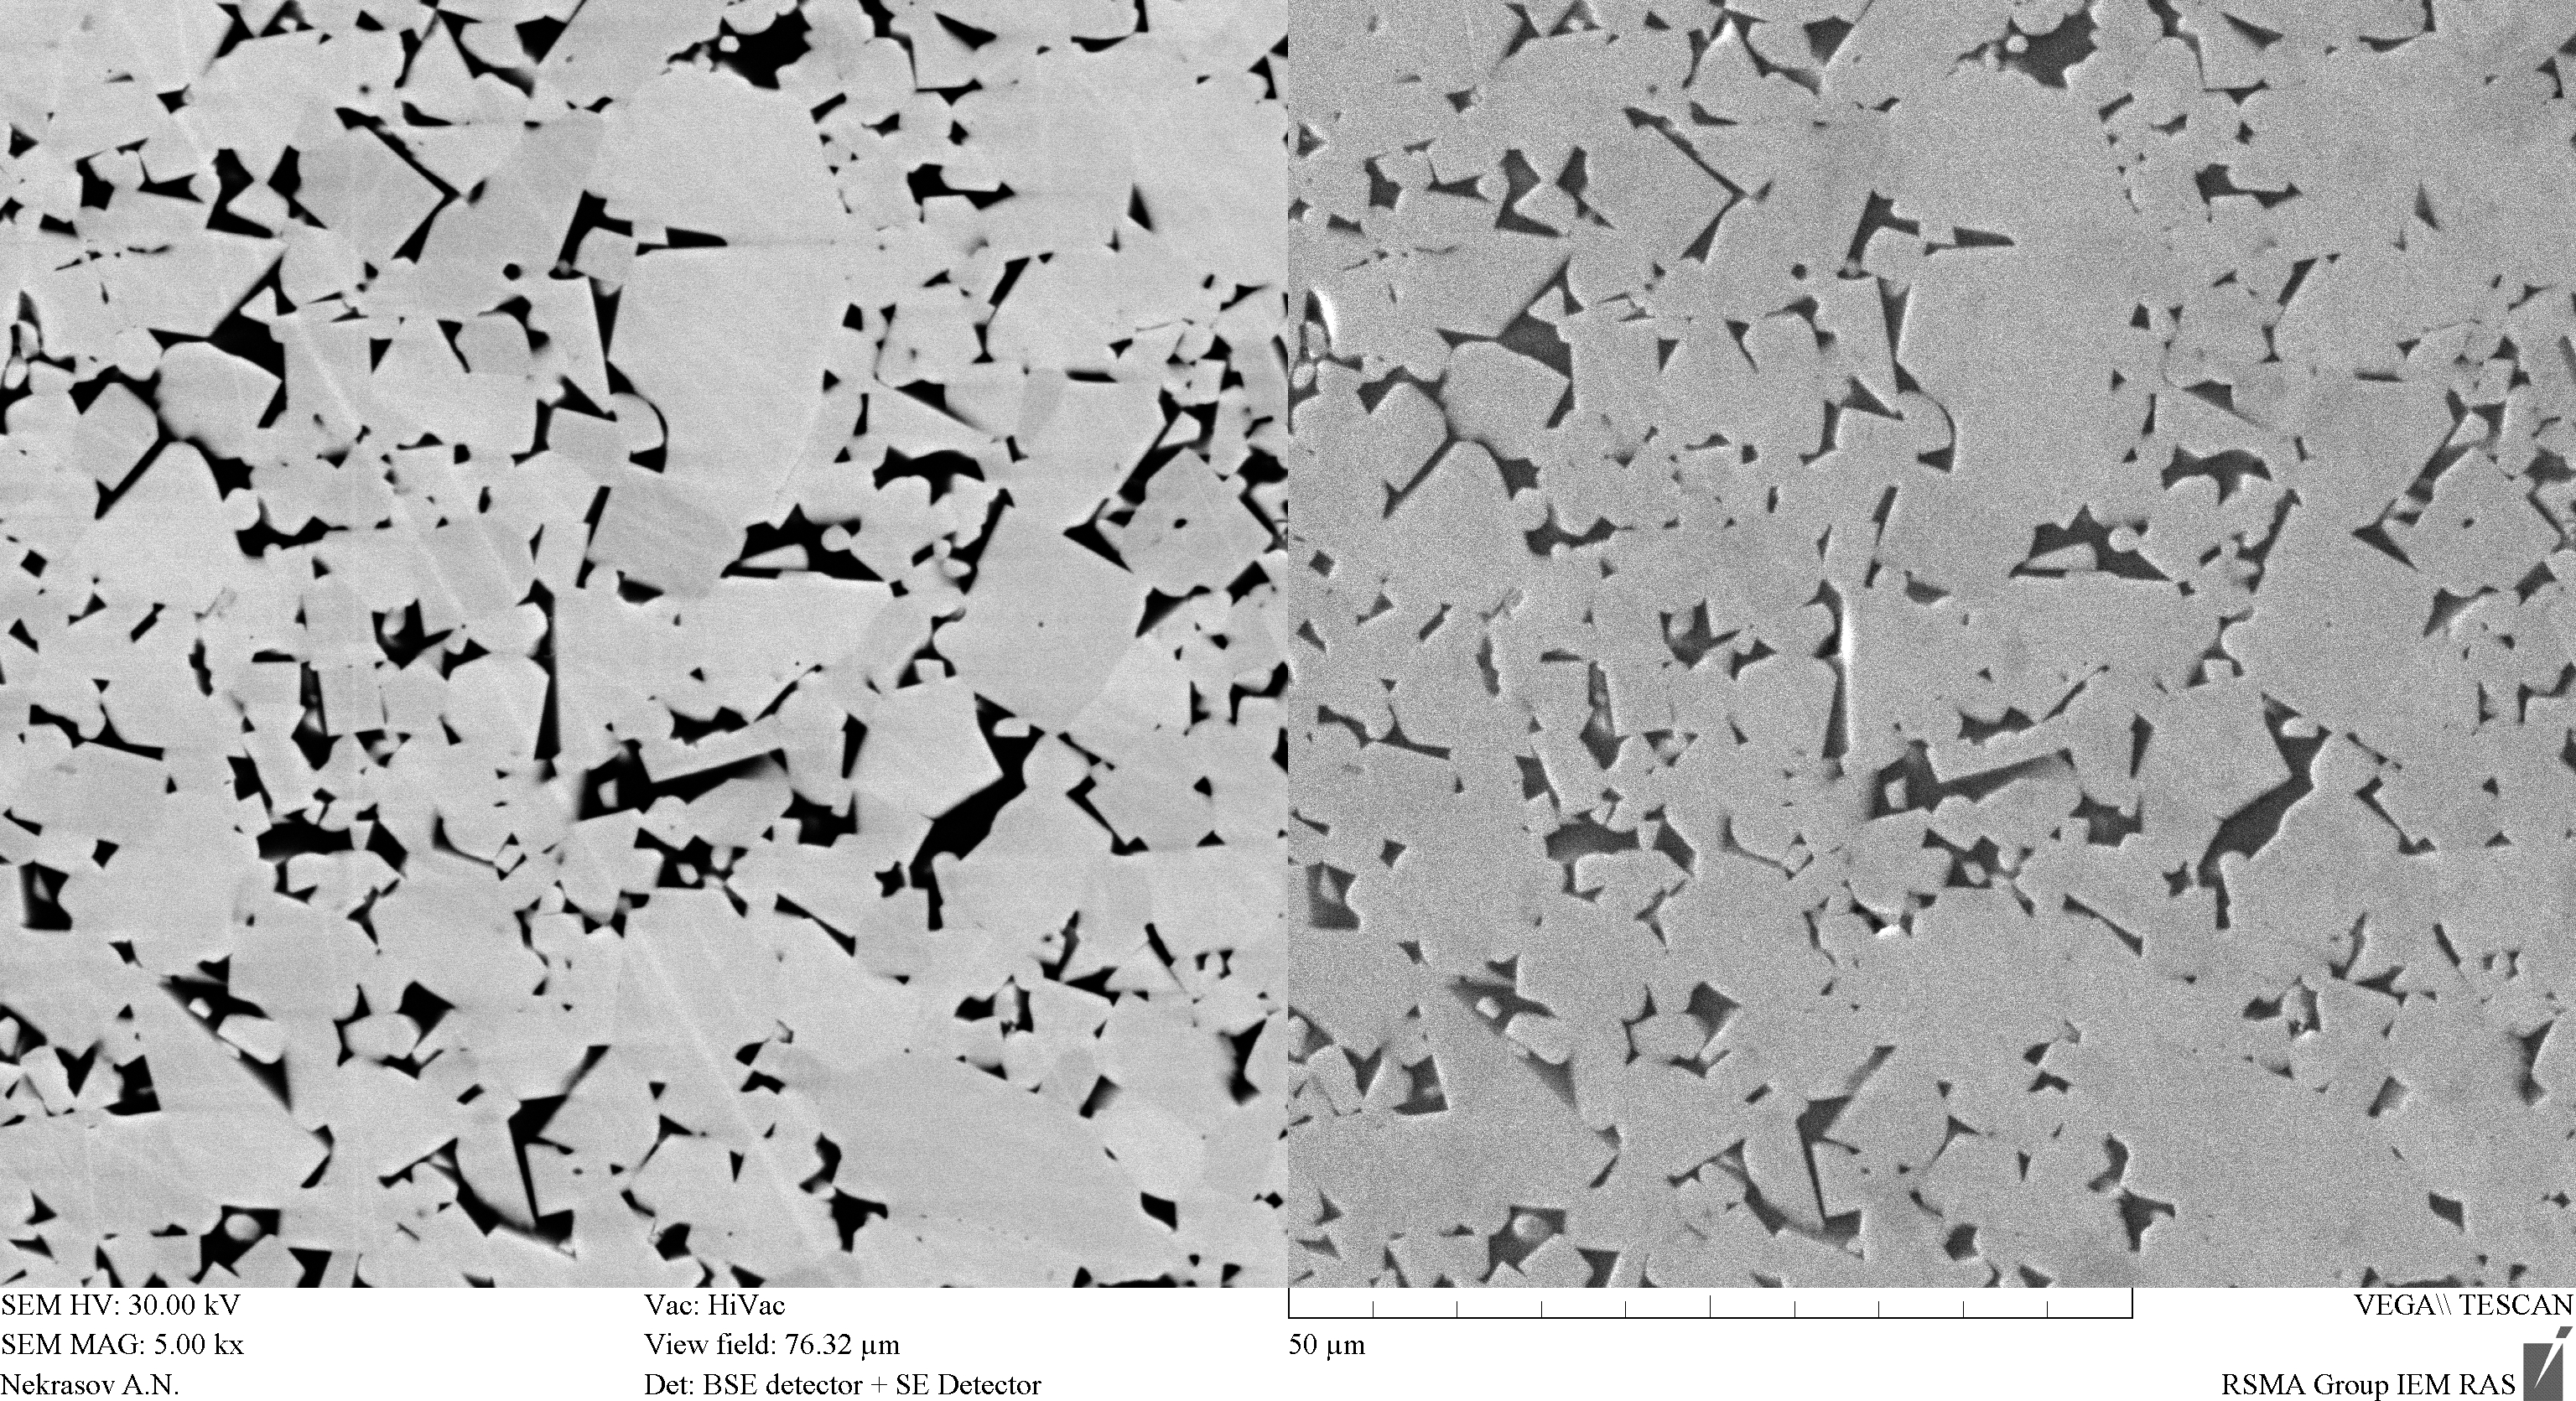
\includegraphics[scale=0.44]{segment_images/original_sem}}
		\caption{полученные в ИФТТ РАН Микроструктуры Wc-Co с помощью электронного сканирующего микроскопа ( “Vega Tescan” )}
		\label{original}
	\end{figure}
	
	Отраженные электроны образуются при рассеивании первичных электронов на большие (до 90º) углы в результате однократного упругого рассеивания или в результате многократного рассеивания на малые углы. В конечном итоге первичные электроны, испытав ряд взаимодействий с атомами образца и теряя при этом энергию, изменяют траекторию своего движения и покидают поверхность образца. Поглощенные электроны. При воздействии зонда часть генерируемых электронов остается в объеме образца. При энергиях первичного пучка 10–20 кэВ примерно 50\% от общего числа образующихся вторичных и отраженных электронов достигают поверхности образца и покидают ее. Оставшиеся электроны образуют ток поглощенных электронов. Разрешающая способность при получении изображений в этом случае имеет такой же порядок, как и для отраженных электронов. Данный метод получения изображений используется редко из-за малой разрешающей способности. Зерно кобальта увидеть нельзя. Количество частичек карбида примерно 300 на одной фотографии.
	
	\subsection{Образование карбидного скелета в сплаве}
	На микроструктурах видно, что образуется «карбидный скелет» так как сплав был получен путем жидкофазного спекания, он будет представлять скелет стянутых зерен карбида вольфрама, а в зазорах расположен в виде сквозной сетки твердый раствор на основе кобальта, пронизывающий пространственный скелет карбида вольфрама. Карбидный скелет (или псевдоскелет) получается потому что почти все границы зерен WC/WC содержат очень тонкие прослойки кобальта с толщиной от одного атомного монослоя до нескольких нанометров. Его наличие показывает, что WC/WC ГЗ характеризуются различными контактными углами с кобальтовой связкой, и только очень
	немногие ГЗ имеют контактные углы, равные нулю. Чистые границы WC/WC, не содержащие кобальтовой прослойки должны быть достаточно хрупкими. 
	
	На начальной стадии спекания карбидных частиц, когда жидкая фаза только что образовалась, имеются три границы: жидкость-газ, твердое тело-газ и жидкость-твердое тело. В этом случае, смачивание WC жидким кобальтом является полным, и уплотнение карбидных частиц до полной плотности происходит очень быстро в результате исчезновения границ жидкость-газ и твердое тело-газ. При этом после завершения начальной стадии спекания в спеченном карбиде вольфрама остаются только границы твердое тело-жидкость, а на границах зерен наблюдается псевдонеполное смачивание. Большие зерна WC растут при  спекании за счет растворения мелких зерен WC. При этом между ними не остается толстых слоев кобальта, как это было бы в случае полного смачивания. Вместо этого, они срастаются вместе, образуя "псевдоскелет", включающий очень тонкие пленки-прекурсоры кобальта в несколько нанометров толщиной. Можно ожидать, что состав пленок-прекурсоров значительно отличается от связки в макроскопических прослойках между зернами WC. В частности, хорошо известно, что тонкие прослойки кобальта, расположенные на границах WC/WC, невозможно удалить при химическом вытравливании кобальта из полностью спеченного карбида.

	\subsection{«Победиты» и технические требования}

	Существует множество сплавов карбида вольфрама, другое их название – «победиты». В зависимости от области применения существуют технические требования к твердым сплавам (рис. \ref{pobedit}).
	
	\begin{figure}[h]
		\center{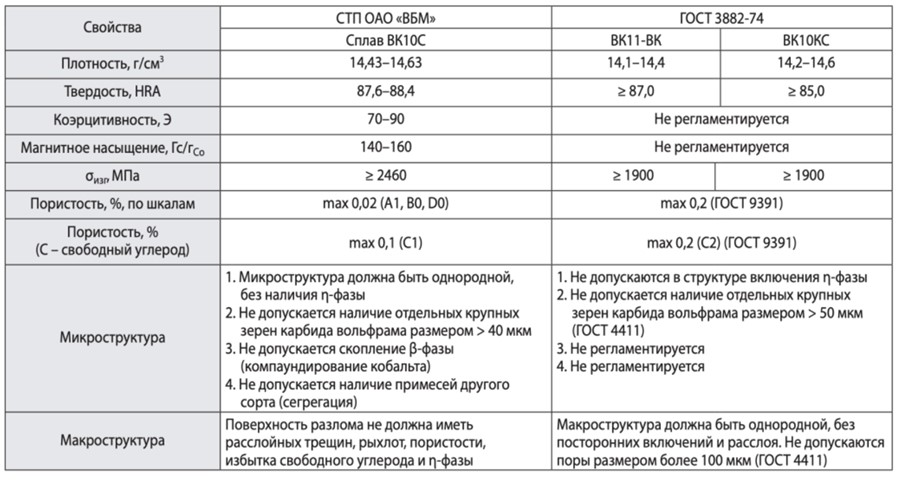
\includegraphics[scale=1]{segment_images/alloy_table1}}
		\caption{Технические требования к сплавам "победит"}
		\label{pobedit}
	\end{figure}
	
	
	По таблице можно узнать допустимый диапазон каждого свойства, эти значения понадобятся нам для сравнения полученных результатов со шкалой нормы. Характеристики исследуемого сплава представлены на рисунке \ref{our_data}.
	
	 \begin{figure}[h]
		\center{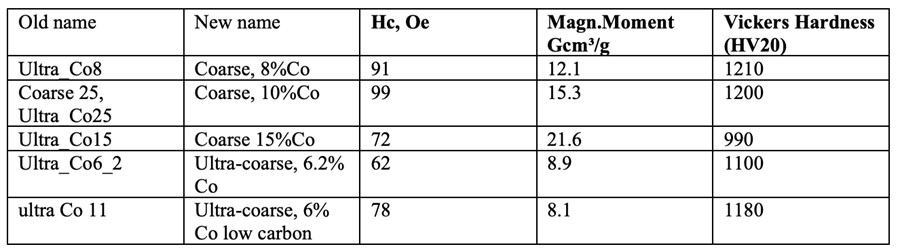
\includegraphics[scale=1.1]{segment_images/alloy_table2}}
		\caption{характеристики сплавов, участвующих в исследовании}
		\label{our_data}
	\end{figure}
	
	\subsection{Обзор литературы}
	Перед началом исследования в первую очередь нужно обратиться к опубликованным ранее работам в сфере обработки изображений микростуктур. 
	
	Этот шаг играет важную роль в работе над проектом. Необходимо понять какие алгоритмы и подходы работают эффективно,а какие лучше не использовать.
	
	\subsubsection{New methods for automatic quantification of microstructural features using digital image processing}
	Andrew Campbell, Paul Murray, Evgenia Yakushina, Stephen Marshall,William Ion. University of Strathclyde, 2018 \cite{dav_abstract_1}.
	
	Поставленная задача - выделение фаз и  пластинчатых колоний на фотографии микроструктуры сплава  Ti6Al4V (сверхпрочный сплав титана, используемый в медицине).
	
	Подход решения задачи - применение на изображении последовательности фильтров и методов. 
	
	\textbf{Сглаживание}. Применение на изображении сглаживающего нормального фильтра. Без него уровень шумов будет неравномерен.
	\textbf{Сегментация}. Использование сегментации Watershed с градиентными маркерами. У сплава  Ti6Al4V ярко выражены смежные границы между фазами и зернами, поэтому карта значений градиентов значительно повысит эффективность сегментации.
	\textbf{Выявление колоний}. В некоторых фазах сплава встречается множество мелких пластинок, направленных в одну сторону. Для их выделения используется карта направлений градиентов изображения, показывающая в какую "сторону" направлен пиксель. Затем при помощи алгоритмов математической морфологии пиксели с схожим направлением группируются в колонию.
	\textbf{Измерения}. В выделенные фазы и колонии вписывается эллипс, по которому определяется гемоетрия региона.
	
	\textbf{Вывод по статье}. Применение сглаживающих фильтров, градиентов изображения и математичсекой морфологии дает хорошую картину при обработке изображений. 
	
	\subsubsection{Measuring Grain Junction Angles in Discretized Microstructures} 
	Michael Chandross, Elizabeth A. Holm. TMS,ASM International,2010 \cite{dav_abstract_2}.
	
	Поставленная задача - провести линейную аппроксимацию границы 3 и более фаз сплава поликристаллического алюминия и посчитать углы регионов в точке соприкосновения.
	
	Подход решения задачи - из точки соединения нескольких фаз провести по границе регионов прямую так, чтобы коэффициент Пирса для нее был максимален. Затем на основе поученных прямых вычислить углы регионов фаз.
	
	\textbf{Выводы по статье}. Хоть структура поликристаллического алюминия сильно отличается от сплава WC-Co, метод аппроксимации границы фаз с помощью коэффициента Пирса может быть полезен.
	
	\subsubsection{The effect of submicron grain size on thermal stability and mechanical properties of high-entropy carbide ceramics
}
	 Fei Wang, Xiang Zhang, Xueliang Yan, Yongfeng Lu, Michael Nastasi, Yan Chen, Bai Cui. University of Nebraska– Lincoln,2020 \cite{dayana_abstract_1}.
	 
	 Уменьшение размера зерна до субмикрометров в керамике значительно улучшает механическую
	 прочность, твердость, трещиностойкость. Главными недостатками при использовании
	 таких структур являются нанокристаллические зёрна, которые становятся нестабильными.
	 
	 Поставленная задача -  изучить природу нестабильных нанокристаллических зерен сплава.
	 
	 \textbf{Ход работы}. Изготовили субмикронные размеры зерна с помощью метода SPS с использованием
	 двухэтапного процесса спекания. Для сравнения результатов эксперимента были
	 использованы крупнозернистые размеры. Для определения размера зерна исследовали
	 поверхности изломов образцов, а также при помощи энергодисперсионного
	 рентгеновского излучения смотрели распределение элементов Ta, Zr, Ti, Nb, Hf и C в двух
	 образцах. Это распределение оказалось близким к стехиометрическому.
	 
	 Предположили,
	 что сложность состава высокой энтропии может снизить энергию границ зерен засчёт
	 увеличения сложности границ зерен. Далее образцы подвергали отжигу при 1300, и 1600
	 градусов цельсия. Крупнозернистый образец проявил более высокую термостойкость, чем
	 мелкозернистый образец. Данный эксперемент позволил предположить, что рост зерен в
	 нанокристаллической керамике может быть замедлен. Завершающим экспериментом было
	 вдавливание в материал четырёхранной алмазной пирамиды (т.е. отпечаток Виккерса).
	 Результат показал, что в крупнозернистом образце вокруг углубления Виккерса
	 произошло сильное растрескивание и вырыв зерна, а в мелкзернистом образце при
	 увеличении стало видно прогиб трещины по границам зёрен. Это является механизмом
	 позволяющим высвободить больше упругой энергии и, таким образом, улучшить
	 сопротивление растрескиванию.
	 
	 \textbf{Выводы}:
	 Кинетика роста зерен в мелкозернистой высокоэнропийной керамике мала при 1300 и
	 1600 ° C, что,возможно, связано со сложностью состава и медленной диффузией.
	 Мелкозернистая высокоэнропийная керамика показала более высокую
	 стойкость к растрескиванию при вдавливании по Виккерсу.
	 Прочность на изгиб и вязкость разрушения мелкозернистых на 25 \% и
	 20 \% соответственно выше, чем у крупнозернистых.
	 
	 \subsubsection{Contact angles of WC/WC grain boundaries with binder in cemented carbides with various carbon content}
	 I.Konyashin, B.B.Straumal, B.Ries, M.F.Bulatov, K.I.Kolesnikov. Element Six GmbH, National University of Science and Technology,Institute of Solid State Physics,Moscow Technological University,2017 \cite{dayana_abstract_2}.
	 
	 Цель работы: выяснение возможного влияния различных состояний границ зерен карбида вольфрама, полностью
	 или не полностью смачиваемых расплавленным Кобальтом в цементированных карбидах WC-Co с различным
	 содержанием углерода.
	 
	 Ход работы: с помощью измельчения, прессования и спекания сверхгрубых порошков карбида вольфрама и
	 добавлением металлического вольфрама или сажи - изготовили специальные образцы со сверхгрубой
	 микроструктурой и низким/высоким содержанием углерода.
	 
	 Чтобы узнать, зависит ли смачиваемость расплавом кобальта от содержания углерода в образце – изготовили
	 специальные образцы разного содержания.
	 Коэрцитивная сила образца с низким содержанием  углерода составила $9.7*10^{-3}$ и его удельное
	  магнитное насыщение составляло 73\%, а сила образца с
	 высоким содержанием углерода составила $6.1*10^{-3}$ и его удельное магнитное насыщение
	 составляло 93\%.
	 
	 Оказалось, что образец с низким содержанием
	 углерода содержит значительно больше малоугловых контактов карбида вольфрама со связующим, чем образец с
	 высоким содержанием углерода. Следовательно, смачиваемость карбида вольфрама жидким связующим на
	 основе кобальта в образце с низким содержанием углерода заметно лучше, чем в образце с высоким содержанием
	 углерода.

	 
	\textbf{Вывод}. различные значения Различные значения смачивания WC / WC GB при различном содержании углерода,
	 по-видимому, являются движущей силой для дрейфа связующего между областями WC-Co с различным
	 содержанием углерода, что позволяет изготавливать функционально-градиентные цементированные карбиды
	 
	\subsection{Анализ современного состояния исследований}
	
	Решение задач в области применения нейронных сетей для поиска и анализа характеристик твердых сплавов не обнаружено. 
	
	Есть множество работ, посвященных приенению глубокого обучения в материловедении, но в большей части из них используются размеченные данные, которых у нас нет. В нашем проекте основная работа связана с созданием алгоритма разметки. 
	
	\section{Актуальность исследования }
	
	Сплав карбида вольфрама кобальтовой связки играет важную роль в горнодобывающей области. На глубине 10 и более километров под землей поломка наплавок бурильной головки создает большую проблему. Чтобы избежать подобных проблем, требуется подробно изучить связку WC-Co и выбрать максимально подходящую под условия комбинацию сплава. Наша работа может помочь раскрыть характеристики сплава и дать более точную информацию для построения математической модели напайной головки.

	\section{Описание использованных подходов }
	Для исследования сплава требуется качественно выделить все характеристики и особенности 
	кристаллической решетки по фотографиям микрострктур. 
	
	Фотографии микростоструктур связки WC-Co имеют видимый уровннь шума. Особенно сильно 
	это видно при оптическом увеличении зерен. Зашумленность выражается в виде 
	множества неупорядоченных белых и серых пикселей на поверхности зерна (рис. \ref{ris:noise}). 
	
	Чтобы снизить уровень шума воспользуемся медианным фильтром. Его особенность в том, что он хорошо справляется со своей задачей и при этом не делает границы объектов менее четкими. 
	
	Также наложим левую и правую части фотографии, чтобы увеличить контрасность признаков (рис. \ref{fig:combine2} ).
	
	\begin{figure}[h]
		\begin{center}
			\begin{minipage}[h]{0.4\linewidth}
				\center{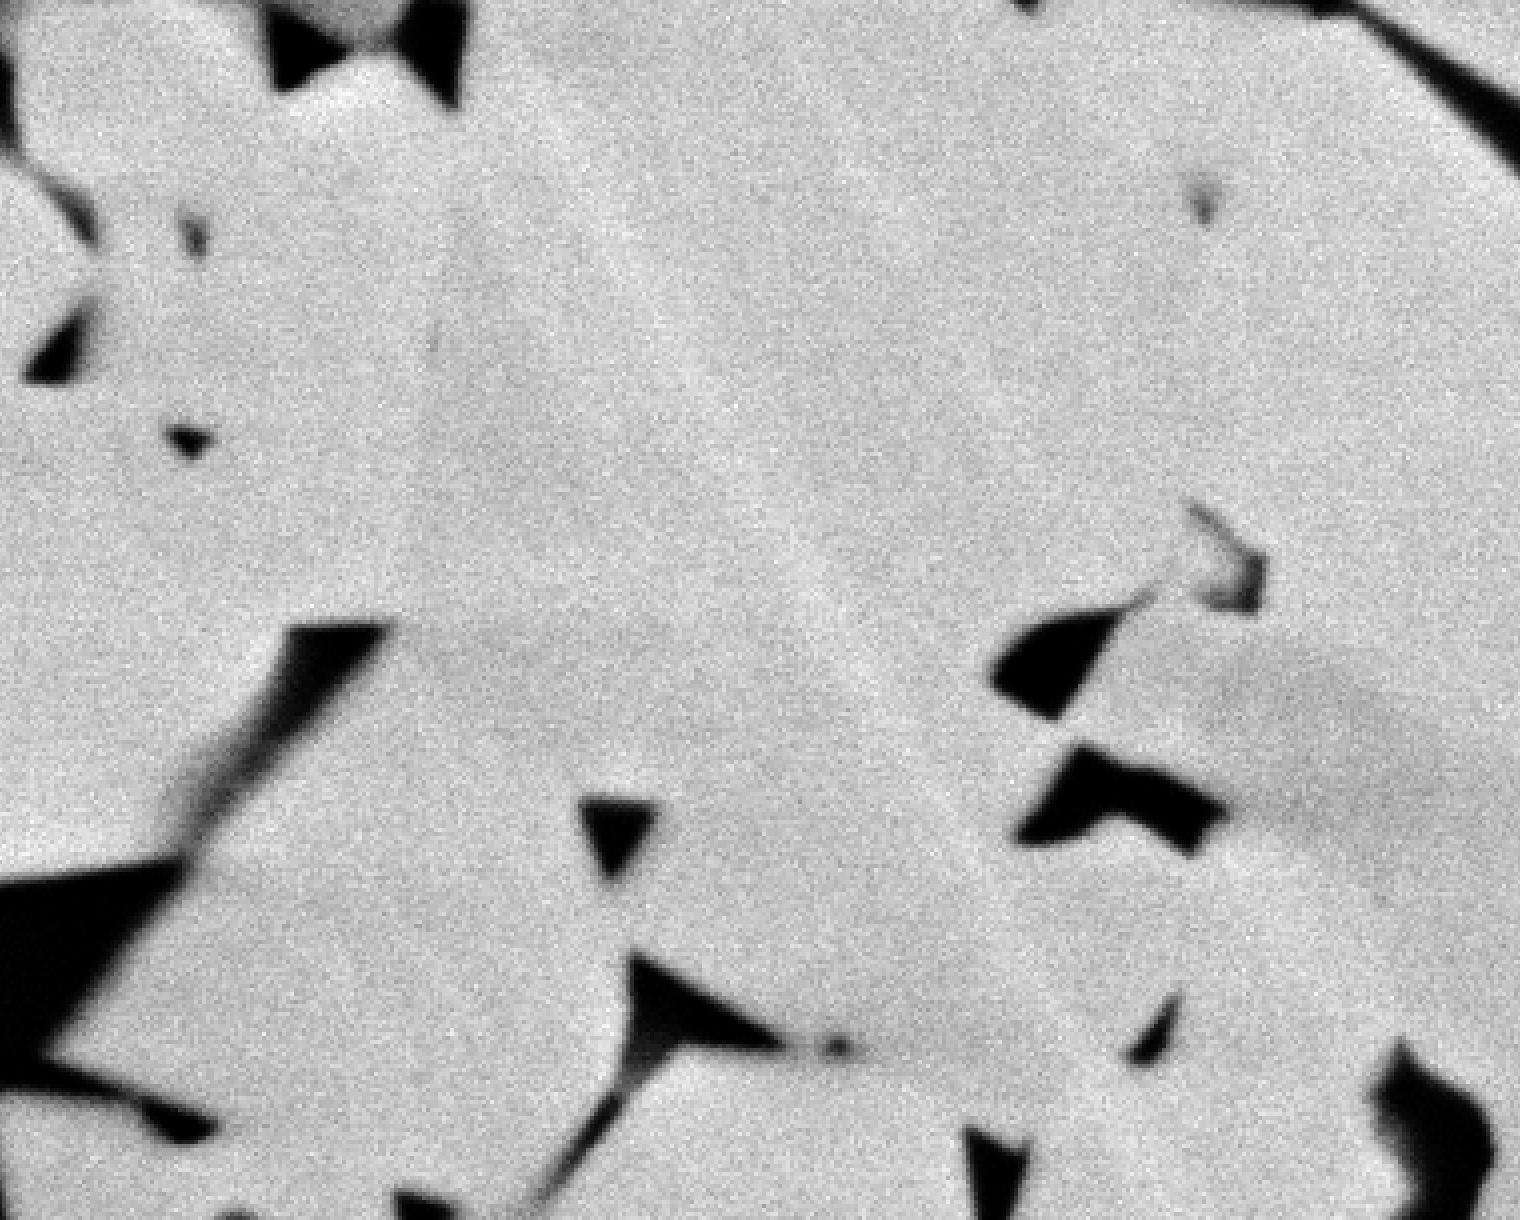
\includegraphics[scale=0.2]{segment_images/grain_zoom}}
				\caption{Зашумленные зерна карбида вольфрама}
				\label{ris:noise}
			\end{minipage}
			\hfill
			\begin{minipage}[h]{0.4\linewidth}
				\center{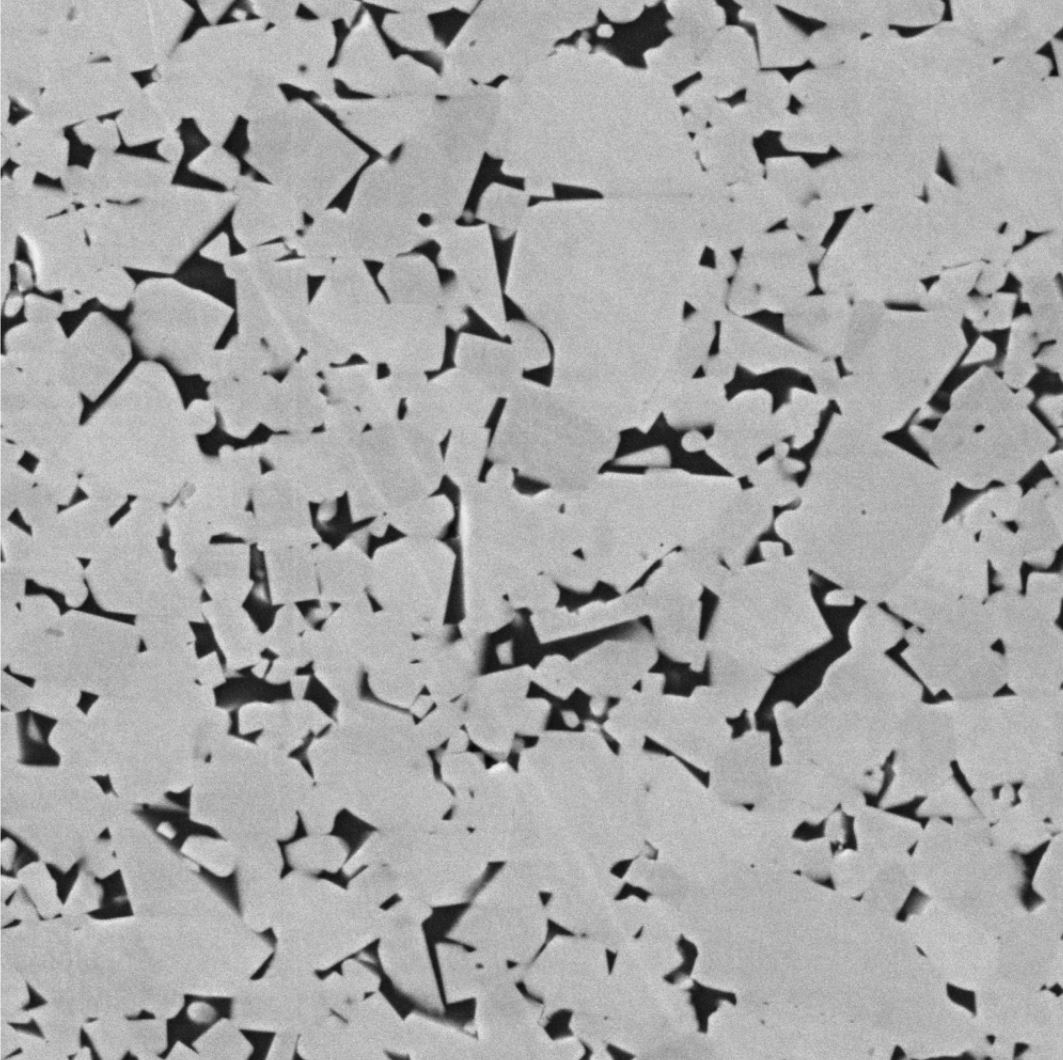
\includegraphics[scale=0.25]{segment_images/combine2}}
				\caption{Совмещенное изображения в поглощенных и отраженных электронах}
				\label{fig:combine2}
			\end{minipage}
		\end{center}
	\end{figure}

	\subsection{Явная сегментация зерен}
	
	Первый подход сбора информации - выделение зерен для сбора их геометрии
	Рассмотрим самые популярные алгоритмы сегментации:
	
	\begin{itemize}
		
		\item  watershed - изображение рассматривается 
		как поверхность \cite{habr_watershed}. Начиная от глобального минимума, изображение будет "заполняться"  водой. 
		По мере поднятия уровня "воды" выделяются локальные минимумы .
		
		Существует также улучшенная версия алгоритма.
		Можно заранее задать прмерные районы минимумов, или иными словами маркеры. 
		Их можно задать вручную, картой расстояний пикселей , 
		картой градиентов  и тд;
		
		\item k-means -  разделение множества входных векторов на группы (кластеры)
		по степени «схожести» друг на друга \cite{habr_k-means}. Алгоритм стремится минимизировать суммарное квадратичное отклонение точек кластеров от центров этих кластеров ; 
		
		\item floodfill -  выделение однородных по цвету регионов при помощи заливки \cite{habr_watershed}. Алгоритм будет объединять пиксели в один сегмент (заливая их одним цветом), если они попадают в указанный диапазон;
		
		\item felzenswalb -  кластеризация минимально охватывающего дерева \cite{felz_link}. 
		Алгоритм не сообщает нам точное количество кластеров, на которые будет разделено изображение. Он будет генерировать столько кластеров, сколько он считает нужным для этого. 
		Применим после метод k-means , это может улучшить качество работы сегментации;
		
		\item DBSCAN - алгоритм группирует вместе точки, которые тесно расположены , помечая как выбросы точки, которые находятся одиноко в областях с малой плотностью \cite{dbscan}.
		
		
	\end{itemize}
	
	Ни один из использованных алгоритмов не смог решить поставленную задачу. Единственный положительный результат - хорошее выделение связующего вещества при помощи watershed с градиентыми маркерами (рис. \ref {fig:watershed_grad}).


	\begin{figure}[h]
		\center{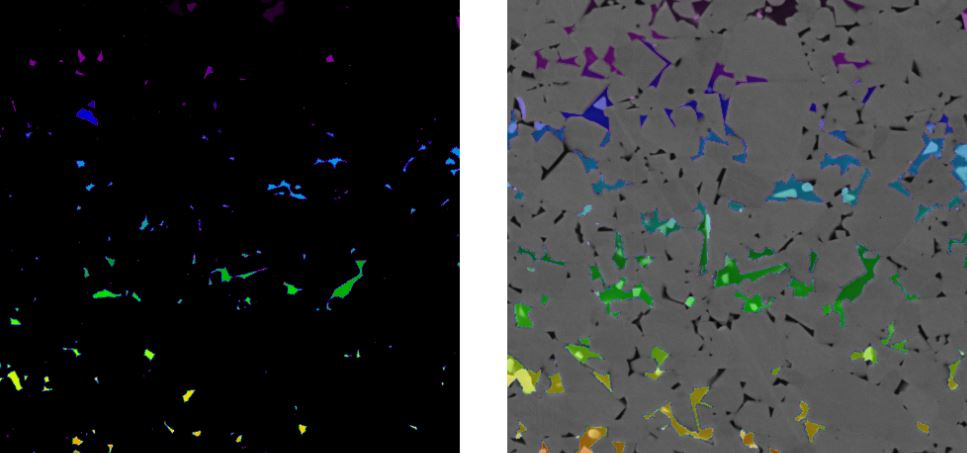
\includegraphics[scale=0.6]{segment_images/watershed_grad}}
		\caption{Watershed с градиентными маркерами}
		\label{fig:watershed_grad}
	\end{figure}

	
	Полученненнй результат можно объяснять тем, что на изображении микроструктуры отчетливо выделены только границы между зернами и  связующим веществом. 
	Видимые границы между смежными зернами отсутвует, из-за чего возникает сложноотделимая масса из
	кристаллов сплава (рис. \ref{marked}). 
	Увеличение контрасности изображения не делает границы зерен более видимыми, а наоборот, значительно 
	повышает уровень шума .
	
	 
	 	\begin{figure}[h]
	 	\begin{center}
	 		\begin{minipage}[h]{0.4\linewidth}
				\center{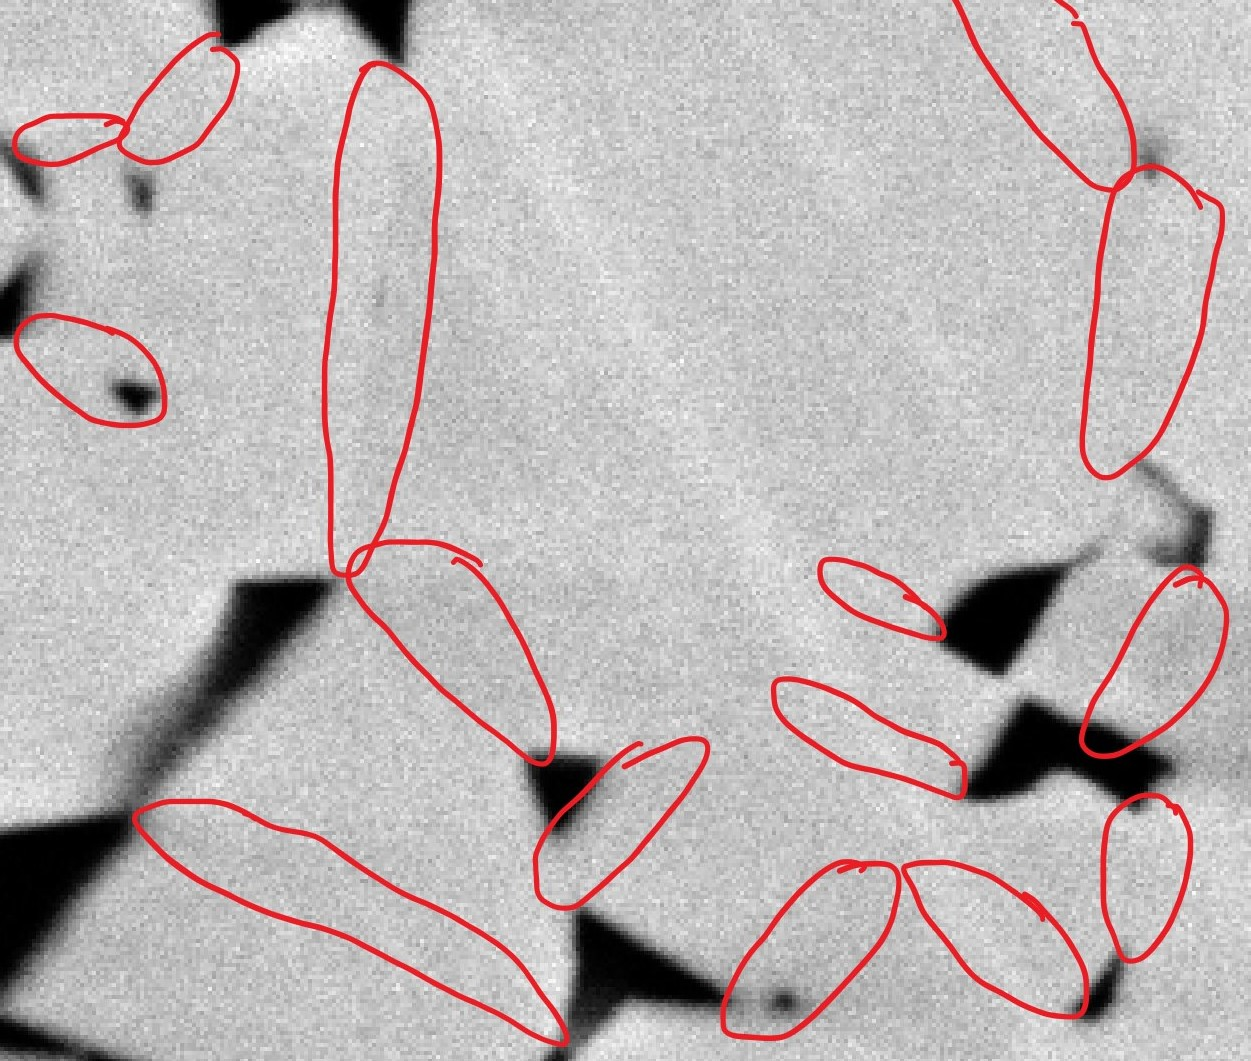
\includegraphics[scale=0.25]{segment_images/grain_zoom_marked}}
				\caption{Красными линиями обведены потенциальные границы смежных зерен}
				\label{marked}
	 		\end{minipage}
	 		\hfill
	 		\begin{minipage}[h]{0.4\linewidth}
				\center{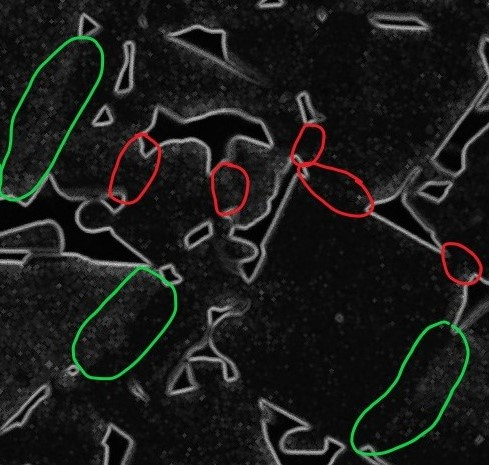
\includegraphics[scale=0.6]{segment_images/grad2_noise_marked}}
				\caption{Зеленой линией отмечено наличие границы, красной линией - отсутсвие границы}
				\label{grad_noise_marked}
	 		\end{minipage}
	 	\end{center}
	 \end{figure}
  
	Большие зерна выделяется на общем фоне уровнем шума, но это неверно для средних и мелких зерен. Если пропустить исходное изображение через детектор границ и контуров \cite{last}, то можно крупные объекты шума можно выделить и соединить их крестиком. Пример такого преобразования  на рисунке \ref{grad_noise_marked}.
	
	
	\subsection{Относительная сегментация зерен}

	Из-за того, сегментация на основе обнаружения границ объектов результата не дали, 
	то попробуем применить другой метод, основанный "пустотах" между зернами.
	
	Выделим все регионы кобальта и аппроксимируем их контуры с помощью линейной функции (рис. \ref{fig:find_contour}).  Для сегментации зерен построим граф G=(V,E), где вершины V - углы периметра региона, а E - ребра, соединяющие вершины.
	Изначально все вершины графа G изолированы. Итеративно пройдемся по всем вершинам, соединяя их друг с другом по специальному правилу (рис. \ref{ris:graph1}).
	Сложность алгоритма заключается в том, что не ясно по какому принципу нужно соединять вершины. Результат графового алгоритма сегментации представлен на рисунке \ref{ris:graph2}
	
	\begin{figure}[h]
		\begin{center}
			\begin{minipage}[h]{0.4\linewidth}
				\center{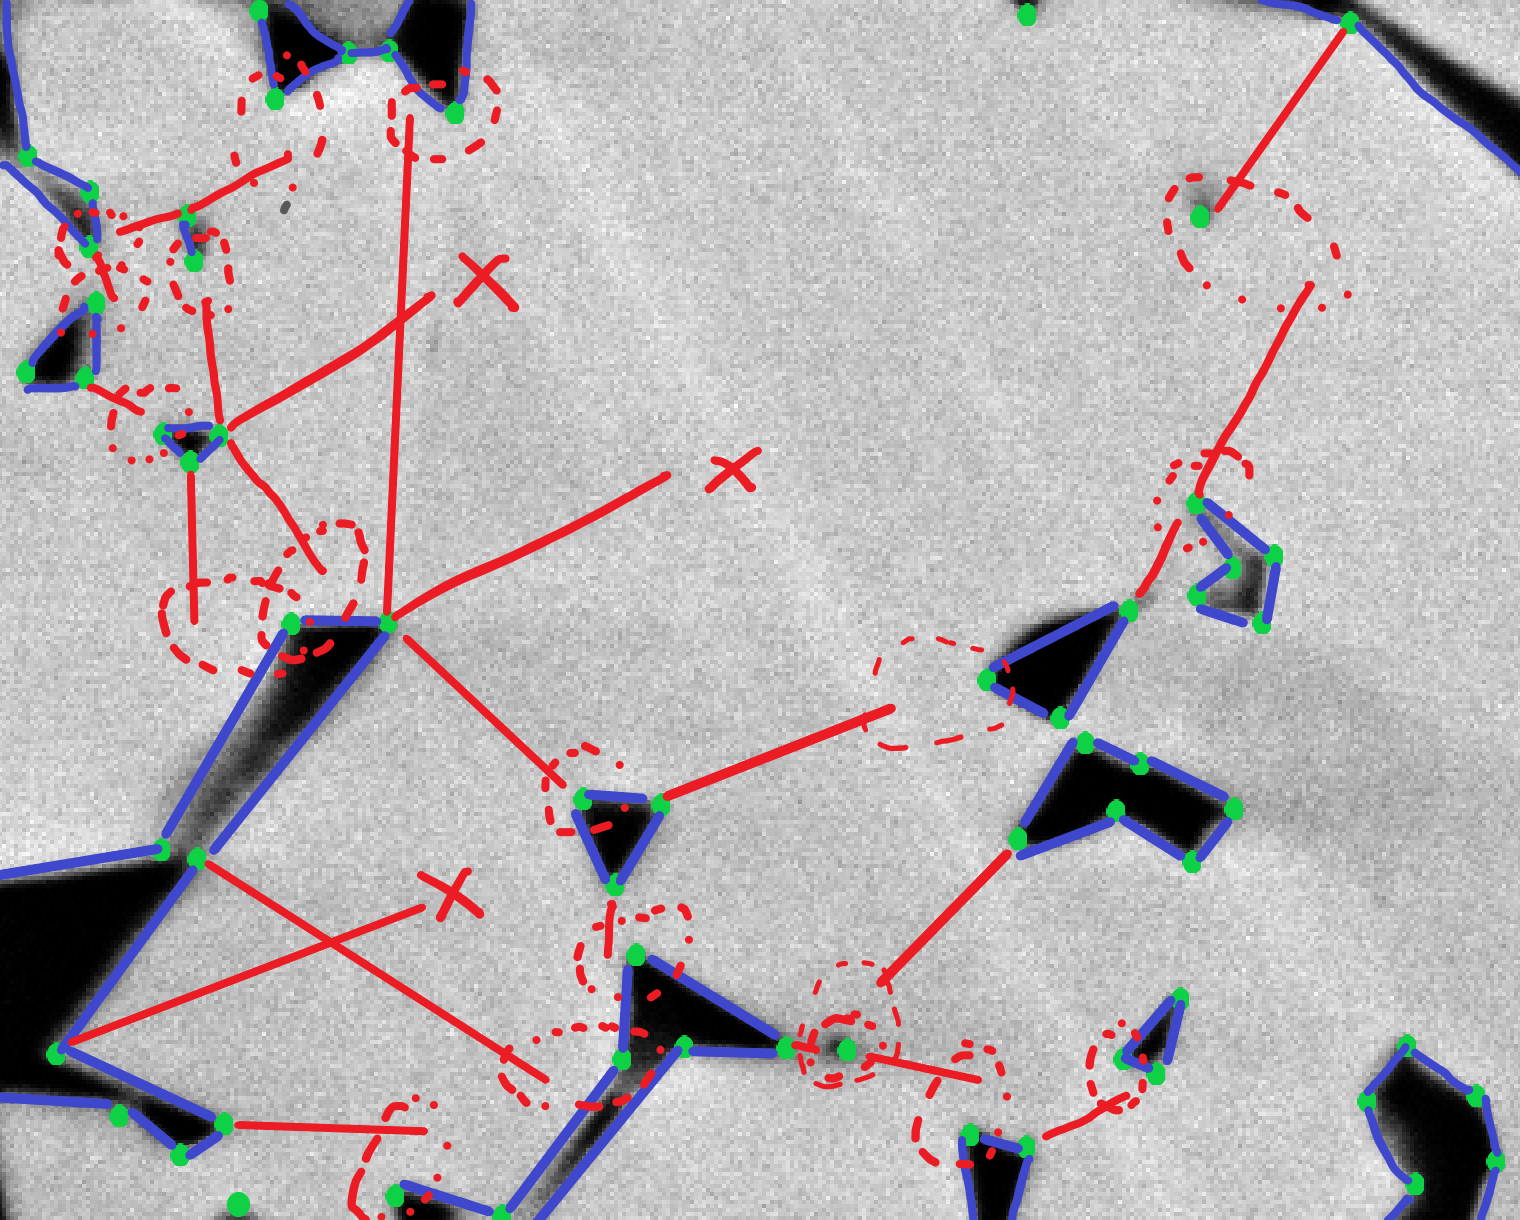
\includegraphics[scale=0.2]{segment_images/zoom_lines_2}}
				\caption{Обход всех вершин и построение дополнительных ребер }
				\label{ris:graph1}
			\end{minipage}
			\hfill
			\begin{minipage}[h]{0.4\linewidth}
				\center{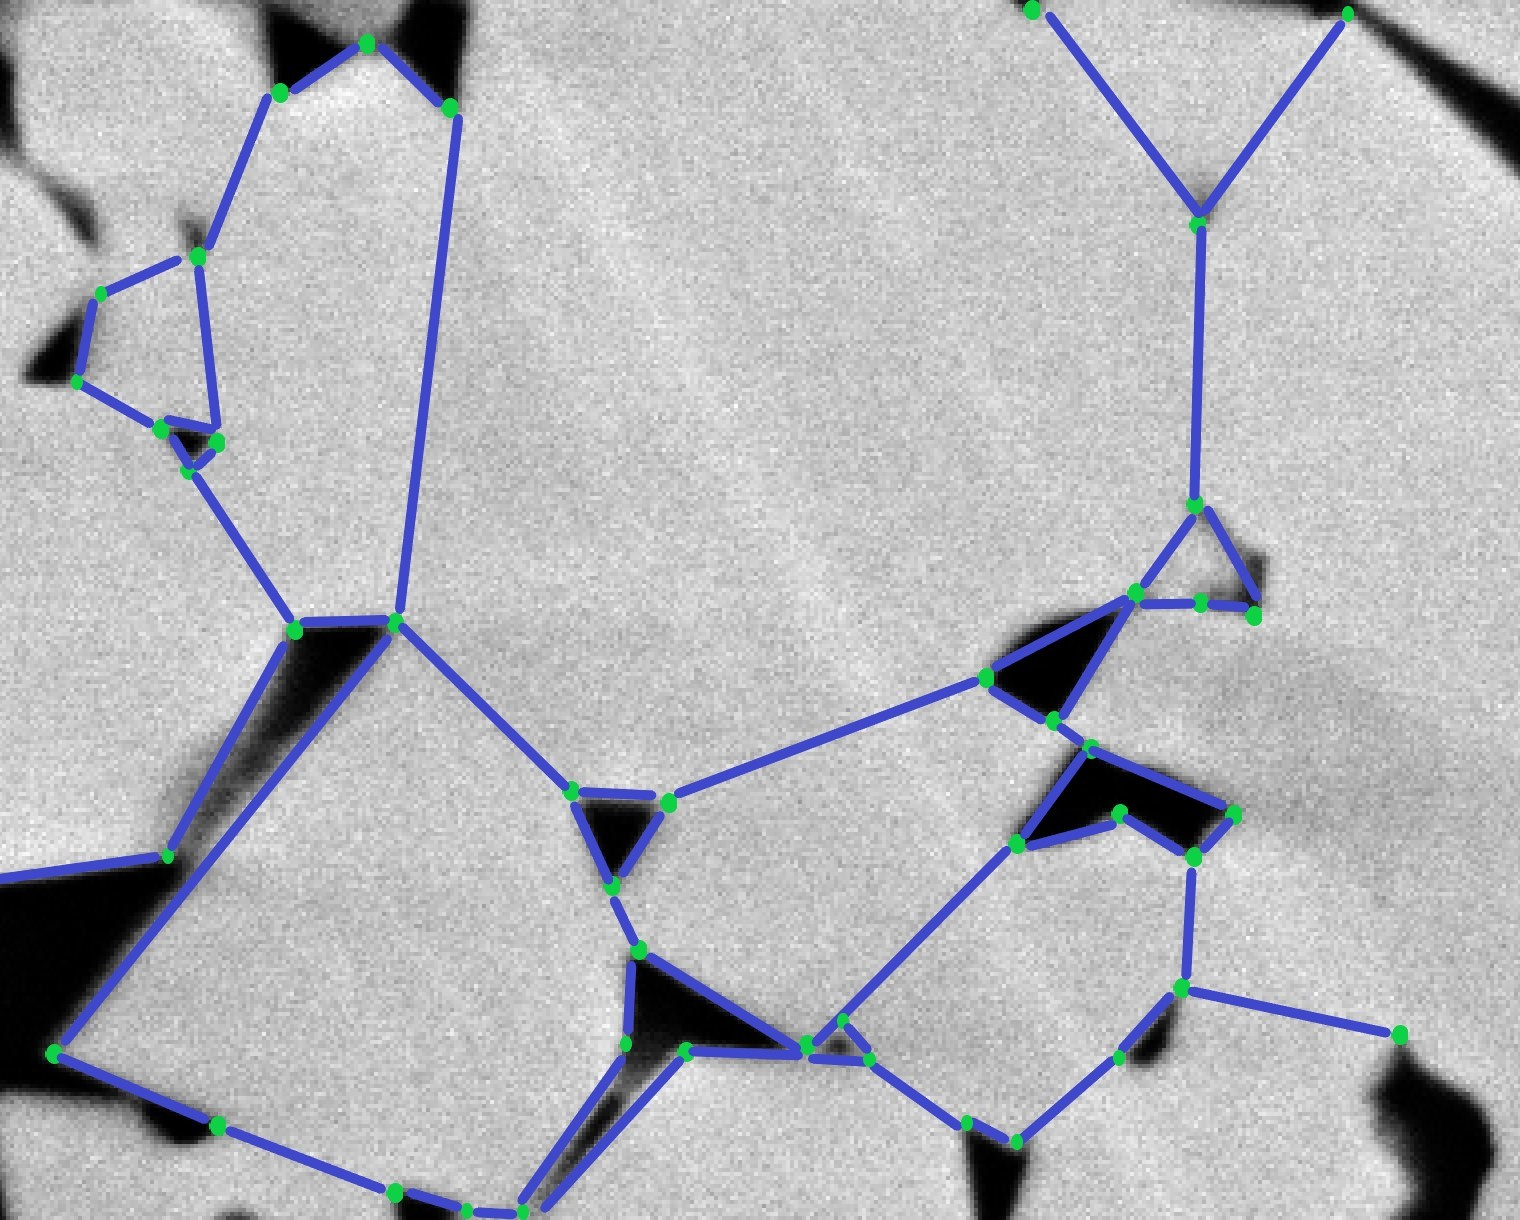
\includegraphics[scale=0.2]{segment_images/grain_zoom_marked_linear}}
				\caption{Получившийся граф G, вершины V - зеленые, ребра E - синие }
				\label{ris:graph2}
			\end{minipage}
		\end{center}
	\end{figure}

	Поставленная задача выделения зерен оказалась нетривиальной. Множество популярных методов не показали достаточный уровень точности определения границы.  
	\newpage
		\subsection{Сегментация связующего вещества}
		
	Воспользуемся иным подходом для сбора геометрии с фотографий микроструктур сплава.Получим упорядоченный набор пикселей контуров регионов кобальта, аппроксимируем их линейной функцией и затем будем собирать информацию по этим регионам. 	
	
	Проведем предобработку изображений.Возьмем только первую половину изображения, полученную на основе отраженных электроов. Самой удачной комбинацией для выделения регионов с кобальтом оказались последовательные шаги
	\begin{itemize}

		\item медианный фильтр; 
		
		\item бинаризация Отсу \cite{otsu}; 
		
		\item карта значений  градиентов.
	\end{itemize}


	Для выделения регионов связующего вещества сплава реализуем последовательность нескольких алгоритмов
	\begin{itemize}
		\item поиск границ детектором Кенни \cite{canny};
		
		\item получение упорядоченного набора пикселей контуров \cite{find_contour};
		
		\item линейная аппроксимация контура \cite{polygon_appx}.
	\end{itemize}
	Сначала детектор границ Кенни выделяет границы у регионов кобальта (рис. \ref{fig:canny}). Затем полученные контуры обрабатываются на алгоритмом \cite{find_contour} и потом каждому пикселю контура присваивается порядковый номер. Последний этап - уменьшение количества точек и аппроксимация пикселей с помощью линейной функции (рис. \ref{fig:find_contour}).
	
	Результат - достаточно точное выделение границ регионов кобальта при помощи прямых линий и отсутсвие необходимости в предварительной разметке углов.
	
	\begin{figure}[h]
		\begin{center}
			\begin{minipage}[h]{0.4\linewidth}
				\center{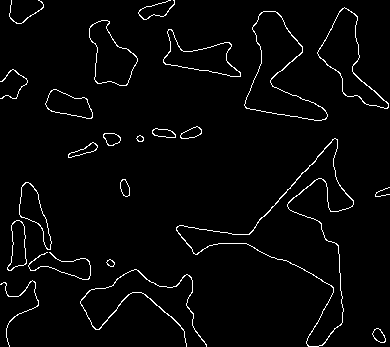
\includegraphics[scale=0.8]{segment_images/edges_resized}}
				\caption{Выделенные методом Кенни контуров кобальта}
				\label{fig:canny}
			\end{minipage}
			\hfill
			\begin{minipage}[h]{0.5\linewidth}
				\center{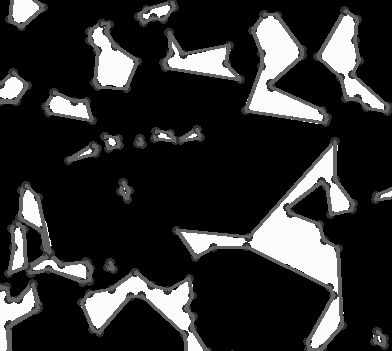
\includegraphics[scale=0.8]{segment_images/lines_resized}}
				\caption{Выделенные регионы связующего вещества с линиями периметра (серые прямые)}
				\label{fig:find_contour}
			\end{minipage}
		\end{center}
	\end{figure}
	
	Метод показал отличное решение поставленной задачи. При помощи комбинации нескольких алгоритмов удалось выделить границы регионов кобальта и получить упорядоченный и линейно приближенный набор пикелей контура.  
	

	
	
	\subsection{Сбор геометрии}
	
	Сегментировать зерна не удалось, поэтому будем работать с регионами связующего вещества. По ним определим следующие характеристики характеристики
	\begin{itemize}
		\item распределение углов;
		
		\item распределение диаметров описанной окружности;
		
		\item распределение дуг максимальной длины в регионе.
	\end{itemize}
	
	Получение распределений углов и диаметров регионов связующего вещества не вызывает сложности, но это не так для получения распределения дуг. 
	Обозначим дугу или медиану сложной фигуры как кусочную линейную функцию, проходящую по точкам медианы треугольников, на которые мы разобьем исходный многоугольник. 
	
	Пусть нужно провести дугу из первого угла региона во второй. Для этого нужно реализовать следующую последовательность алгоритмов 
	\begin{itemize}
		\item триангуляция многоугольника;
		
		\item поиск точек медиан на сторонах треугольников, которые находятся внутри региона;
		
		\item создание графа из точек медиан и соединение их ребрами так, чтобы ребро находилось внутри региона. Возможно  для этого пункта подойдет триангуляция Делоне;
		
		\item поиск кратчайшего пути в графе из исходной вершины угла в заданную.
	\end{itemize}
	
	Указанный алгоритм еще нереализован, но при анализе (рис. \ref{arc}) показал хорошие перспективы в решении задачи сбора геометрии регионов связующего вещества сплава.
	
	\begin{figure}[h]
		\center{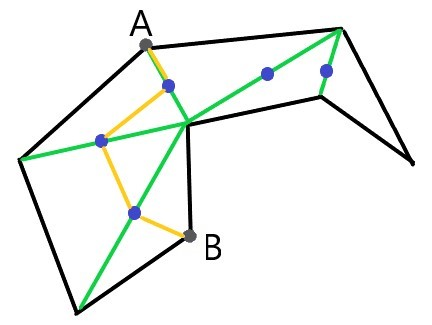
\includegraphics[scale=0.99]{segment_images/arc}}
		\caption{Возможный результат построения дуги}
		\label{arc}
	\end{figure}
	
	
	\section{Обсуждение полученных результатов }
	
	Инициатором и соруководителем проекта является профессор Б.Б.Страумал. Под его руководством были созданы и отправлены нам снимки микроструктур сплава WC-C.
	
	На последней онлайн-встрече мы получили от Бориса Борисовича положительный отзыв касательно нашей работы.
	
	
	\section{Результаты}
	
	Проведен анализ микроструктур сплава  WC-Co. Определены измененения  характеристик сплава при изменении размера зерен. 
	
	Разработана методика сбора геометрии по регионами связующего вещества.
	
	

	



\newpage
%далее сам список используевой литературы
\begin{thebibliography}{}
	
	
	\bibitem{last}  Каграманян Д.Г. -  Cегментации пустот сплава WC-Co
			\bibitem{habr_watershed}  NastyaL  -  \href{https://habr.com/ru/company/intel/blog/266347/}{Обзор алгоритмов сегментации}
	\bibitem{habr_k-means} sashaeve - 
	\href{https://habr.com/ru/post/67078/}{Кластеризация: алгоритмы k-means и c-means}
	\bibitem{felz_link}  Pedro F. Felzenszwalb, Daniel P. Huttenlocher  -  
	\href{https://people.cs.uchicago.edu/~pff/papers/seg-ijcv.pdf}{Efficient Graph-Based Image Segmentation}
	\bibitem{dbscan} Siarshai
	- \href{https://habr.com/ru/post/322034/}{Интересные алгоритмы кластеризации, часть вторая: DBSCAN}
	
		\bibitem{ndi_label}   \href{https://docs.scipy.org/doc/scipy/reference/generated/scipy.ndimage.label.html}{scipy.ndimage.label}
	
	\bibitem{polygon_anal}  Hongyun Zhang ,Quanhua Zhao  ,Yu Li   -  \href{https://journals.plos.org/plosone/article?id=10.1371/journal.pone.0230342}{Generation of simple polygons from ordered points using an iterative insertion algorithm}
	
	\bibitem{convex_hull}    \href{https://en.wikipedia.org/wiki/Convex_hull}{Convex hull}
	
	\bibitem{corners}  Shi-Tomasi   -  \href{https://en.wikipedia.org/wiki/Corner_detection}{Corner detection}
	
	\bibitem{polygon_appx} Ramer,Douglas,Peucker  - \href{https://habr.com/ru/post/448618/}{Ramer–Douglas–Peucker algorithm}
	
	\bibitem{skimage_approx}  \href{https://scikit-image.org/docs/dev/auto_examples/edges/plot_polygon.html#sphx-glr-download-auto-examples-edges-plot-polygon-py} {Approximate and subdivide polygons}
	
	\bibitem{detectors} lightsource
	-  \href{	https://habr.com/ru/post/244541/} {Детекторы углов}
	
	\bibitem{otsu}  Nobuyuki Otsu - \href{https://en.wikipedia.org/wiki/Otsu%27s_method} {Otsu's method}
	
	
	\bibitem{david} Д.Г.Каграманян -  Сегментация зерен сплава WC-Co готовыми инструментами
	
	\bibitem{line}   Брезенхэм   -  \href{https://en.wikipedia.org/wiki/Bresenham%27s_line_algorithm}{Отрисовка линий в двумерного растра}
		
	\bibitem{canny}    John F. Canny    -  \href{https://en.wikipedia.org/wiki/Canny_edge_detector}{Canny edge detector}
	
	\bibitem{canny_habr}   impersonalis   -  \href{https://habr.com/ru/post/114589/}{Выделение границ Канни}
	
	\bibitem{find_contour}  Satoshi Suzuki,Keiichi Abe   -  \href{https://www.sciencedirect.com/science/article/abs/pii/0734189X85900167}{Topological Structural Analysis of Digitized Binary Images by Border Following}
	
	\bibitem{dav_abstract_1}  Andrew Campbell, Paul Murray, Evgenia Yakushina, Stephen Marshall,William Ion   -  \href{https://www.sciencedirect.com/science/article/pii/S0264127517311620}{New methods for automatic quantification of microstructural features using digital image processing}
	
	\bibitem{dav_abstract_2} Michael Chandross, Elizabeth A. Holm   -  \href{https://link.springer.com/article/10.1007%2Fs11661-010-0355-7}{Measuring Grain Junction Angles in Discretized Microstructures}
		
	\bibitem{dayana_abstract_1} Fei Wang, Xiang Zhang, Xueliang Yan, Yongfeng Lu, Michael Nastasi, Yan Chen, Bai Cui  -  \href{https://ceramics.onlinelibrary.wiley.com/doi/abs/10.1111/jace.17103}{The effect of submicron grain size on thermal stability and mechanical properties of high‐entropy carbide ceramics}
	
	\bibitem{dayana_abstract_2} I.Konyashin, B.B.Straumal, B.Ries, M.F.Bulatov, K.I.Kolesnikov   -  \href{https://www.sciencedirect.com/science/article/abs/pii/S0167577X17303361}{Contact angles of WC/WC grain boundaries with binder in cemented
		carbides with various carbon content}
		
	\bibitem{dayana_abstract_3} Fei Wang, Xiang Zhang, Xueliang Yan, Yongfeng Lu, Michael Nastasi, Yan Chen, Bai Cum   -  \href{https://ceramics.onlinelibrary.wiley.com/doi/abs/10.1111/jace.17103}{The effect of submicron grain size on thermal stability and mechanical properties of high‐entropy carbide ceramics}

\end{thebibliography}




	
\end{document}